% =================================================================================
\section{Approximation numérique préliminaire}\label{Chapitre_3}
% =================================================================================
Dans cette section nous allons étudier numériquement le problème de Rayleigh-Stokes en $1$D sur le segment $[0, L]$ où $L>0$ est un réel que l'on précisera lors de l'implémentation de quelques cas tests. On va considérer le problème suivant
\begin{equation*}
\begin{cases}
    \partial_tu(t,x) - \nu\partial_{xx} u(t,x) - \alpha\partial_{xxt} u(t,x) = f & \forall (t,x) \in  \bbR_+^* \times \ ]0,L[  \\
    u(0,x) = u_0(x) & \forall x \in \ ]0,L[ \\
    u(t, 0) = u(t,L) = 0 & \forall t \in \bbR_+^*
\end{cases}
\end{equation*}
Tout comme le réel $L$, on précisera la donnée initiale $u_0$ et le second membre $f$ lors de l'implémentation des cas tests. Nous allons approcher ce problème par une méthode différence finie.

\subsection{Définition du schéma différence finie}
Commençons par la discrétisation spatiale. Soit $m \in \bbN^*$ le nombre de maille. On pose $h = \dfrac{L}{m+1}$ le pas d'espace et $x_i = ih$ les noeuds du maillage de sorte que
\begin{center}
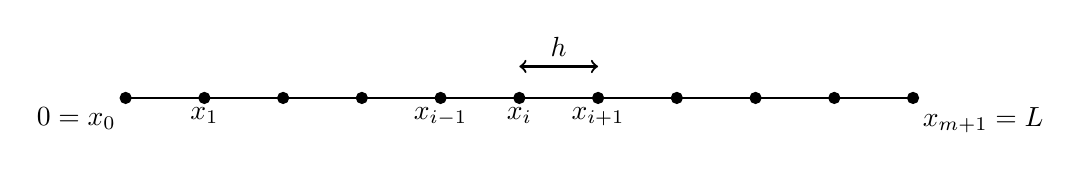
\begin{tikzpicture}
    % Ligne horizontale
    \draw[thick] (0,0) -- (10,0);
    % Positions des noeuds
    \foreach \x in {0, 1, 2, 3, 4, 5, 6, 7, 8, 9, 10}
    \filldraw[black] (\x, 0) circle (2pt);
    % Flèche double pour h
    \draw[<->, thick] (5,0.4) -- (6,0.4) node[midway, above] {$h$};
    % Labels en dessous
    \node[below left] at (0, 0)  {$0 = x_0$};
    \node[below] at (1, 0)  {$x_1$};
    \node[below] at (4, 0)  {$x_{i-1}$};
    \node[below] at (5, 0)  {$x_i$};
    \node[below] at (6, 0)  {$x_{i+1}$};
    \node[below right] at (10, 0) {$x_{m+1} = L$};
\end{tikzpicture}
\end{center}
On va approché $\partial_{xx}$ par l'opérateur approché à trois noeuds
\begin{equation*}
    \Delta_hu(t,x) = \frac{u(t,x-h)-2u(t,x)+u(t,x+h)}{h^2}
\end{equation*}
On note $u_h$ la solution numérique et on veut calculer cette solution aux point $x_i$, on pose $u_i(t)=u_h(t,x_i)$ et $f_i=f(x_i)$. On obtient le schéma semi-discret
\begin{equation}\label{schema_semi_discret}
    \partial_tu_i(t)-\nu\frac{u_{i-1}(t)-2u_i(t)+u_{i+1}(t)}{h^2}-\alpha\frac{\partial_tu_{i-1}(t)-2\partial_tu_i(t)+\partial_tu_{i+1}(t)}{h^2}=f_i
\end{equation}
On passe ensuite à la discrétisation temporelle. Soit $T>0$ le temps final. On partitionne $[0,T]$ en introduisant les instants $t_n = n \Delta t$, où $\Delta t$ est le pas de temps qui sera défini plus tard. On note à présent $u_i^n=u_h(x_i,t_n)$ l'approximation de la solution $u(x,t)$ au point $x_i$ et à l'instant $t_n$. On va utiliser le schéma d'Euler implicite pour l'approximation temporelle, donc on intègre \eqref{schema_semi_discret} entre deux instants $t_n$ et $t_{n+1}$, et on utilise la méthode des rectangles à droites pour approximer les intégrales. Ce qui nous donne après avoir divisé par $\Delta t$
\begin{equation}\label{schema_DF_points}
    \frac{u_i^{n+1}-u_i^n}{\Delta t} - \nu \frac{u_{i-1}^{n+1}-2u_i^{n+1}+u_{i+1}^{n+1}}{h^2} - \frac{\alpha}{\Delta t}\bigg( \frac{u_{i-1}^{n+1}-2u_i^{n+1}+u_{i+1}^{n+1}}{h^2}-\frac{u_{i-1}^{n}-2u_i^{n}+u_{i+1}^{n}}{h^2}\bigg) = f_i
\end{equation}
Notons à présent $U^n$ le vecteur solution à l'instant $n$, $\Delta_h$ la matrice de discrétisation de la dérivée seconde en espace et $F$ le vecteur second membre, respectivement définis par 
\begin{eqnarray*}
    U^n = \begin{pmatrix}
        u_0^n \\
        \vdots \\
        u_{m+1}^n
    \end{pmatrix}, \ \ \ F=\begin{pmatrix}
        f_0 \\
        \vdots \\
        f_{m+1}
    \end{pmatrix} \ \ \ &\text{ et }& \ \ \ 
    \Delta_h = \frac{1}{h^2}\begin{pmatrix}
        -2 & 1 & 0 & \cdots & \cdots & 0 \\
        1 & -2 & 1 & \ddots &  & \vdots \\
        0 & 1 & -2 & 1 & \ddots & \vdots \\
        \vdots & \ddots & \ddots & \ddots & \ddots & 0 \\
        \vdots &  & \ddots & \ddots & \ddots & 1 \\
        0 & \cdots & \cdots & 0 & 1 & -2 
    \end{pmatrix}
\end{eqnarray*}
On peut ainsi réécrire l'équation précédente de la façon suivante
\begin{eqnarray*}
    \frac{U^{n+1} - U^n}{\Delta t} - \nu \Delta _h U^{n+1} - \alpha\bigg(\frac{\Delta_h U^{n+1} - \Delta_h U^n}{\Delta t} \bigg) = F
\end{eqnarray*}
En réorganisant les termes pour isoler l'inconnue au temps $n+1$, nous obtenons le système 
\begin{eqnarray}\label{schema_DF}
    \big(I - (\nu \Delta t + \alpha)\Delta_h\big)  U^{n+1} = (I - \alpha \Delta_h) U^n + \Delta t F
\end{eqnarray}
où $I$ désigne la matrice identité. On peut maintenant s'intéresser aux propriétés de ce schéma.

\subsection{Propriétés du schéma}
\subsubsection{Consistance}
On étudie l'erreur de troncature $\tau_h := \calL_hu - \calL u$ où
\begin{eqnarray*}
    \calL u(t,x) &=& \partial_tu(t,x) - \nu \partial_{xx}u(t,x)-\alpha\partial_{xxt}u(t,x) \\
    && \\
     \calL_hu(t,x) &=& \frac{u(t+\Delta t,x)-u(t,x)}{\Delta t}-\frac{\alpha}{\Delta t}\bigg(\frac{u(t+\Delta t,x-h)-2u(t+\Delta t, x)}{h^2} \\
     &+& \frac{u(t+\Delta t, x+h)}{h^2}-\frac{u(t,x-h)-2u(t, x)+u(t, x+h)}{h^2}\bigg)\\ 
     &-& \nu \frac{u(t+\Delta t,x-h)-2u(t+\Delta t, x)+u(t+\Delta t, x+h)}{h^2}  
\end{eqnarray*}
Pour plus de lisibilité posons,
\begin{eqnarray*}
    A &:=& \frac{u(t+\Delta t,x)-u(t,x)}{\Delta t} \\
    B &:=&  \nu \frac{u(t+\Delta t,x-h)-2u(t+\Delta t, x)+u(t+\Delta t, x+h)}{h^2} \\
    C &:=& \frac{\alpha}{\Delta t}\bigg(\frac{u(t+\Delta t,x-h)-2u(t+\Delta t, x) + u(t+\Delta t, x+h)}{h^2} \\
    &-&\frac{u(t,x-h)-2u(t, x)+u(t, x+h)}{h^2}\bigg)
\end{eqnarray*}
On calcule donc $\tau_h$ en effectuant des développements limités et on obtient
\begin{eqnarray*}
    A &=& \partial_{t}u(t,x) - \frac{\Delta t}{2} \partial_{tt}u(t,x) + O(\Delta t^2) \\
    B &=&  \nu \Big(\partial_{xx}u(t,x) + \frac{h^2}{12} \partial_{xxxx}u(t,x) + O(h^3)\Big) \\
    C &=& \alpha\Big(\partial_{xxt}u(t,x) + \frac{h^2}{12}\partial_{xxxxt}u(t,x) - \frac{\Delta t}{2}\partial_{xxtt}u(t,x) \\
    &-& \frac{h^2\Delta t}{24}\partial_{xxxxtt}u(t,x) + O(\Delta t^2 + h^3)\Big)   
\end{eqnarray*}
D'où 
\begin{eqnarray*}
    \calL_hu -\calL u &=& -\frac{\Delta t}{2}\partial_{tt}u - \nu \frac{h^2}{12}\partial_{xxxx}u - \alpha\frac{h^2}{12}\partial_{xxxxt}u \\
    &+& \alpha\frac{\Delta t }{2}\Bigl(\partial_{xxtt}u + \frac{h^2}{12}\partial_{xxxxtt}u \Bigl) + O(\Delta t^2 + h^3) \\
    &=& O(\Delta t + h^2)
\end{eqnarray*}
Le schéma est consistant d'ordre 1 en temps et d'ordre 2 en espace.

\subsubsection{Stabilité}\label{Stabilité_EI}
Le problème de Rayleigh-Stokes est extrêmement stable. L'analyse suivante va permettre de mettre en évidence le caractère stable en temps long du schéma mais aussi la propriété de filtre passe-bas que possède $\alpha$. Nous allons étudier la stabilité $L^2$ du schéma par une analyse de Fourier. Il est cependant nécessaire de faire l'hypothèse que la solution est périodique, cela revient à étudier la stabilité du schéma loin des bords. On définit $u_h$ par
\begin{eqnarray*}
    u_h(t,x) = u_i^n \ \ \ &\text{ si }& \ \ \ \left\{\begin{array}{l}
        x \in \big[\max(x_i-\frac{h}{2},0), \min(x_i+\frac{h}{2},L)\big[ \\
        t \in [t_n,t_{n+1}[
    \end{array}\right.
\end{eqnarray*}
Ainsi, $u_h$ est une fonction constante par morceaux. On fait l'hypothèse que $u_h$ est périodique de période $L$. On peut alors décomposer $u_h(t_n,\cdot)$ en somme de Fourier
\begin{equation*}
    u_h(t_n,x)=\sum_{k \in \bbZ} \hat{u}(k)\ex^{2\pi i kx}
\end{equation*}
où les moments sont définis par
\begin{equation*}
    \hat{u}^n(k)=\int_0^Lu_h(t_n,x)\ex^{-2\pi ikx}\mathrm{d}x
\end{equation*}
On va réécrire le schéma \eqref{schema_DF_points} de manière à avoir les inconnues au temps $t_{n+1}$ d'un côté de l'égalité et les inconnues au temps $t_n$ de l'autre. Pour l'étude de la stabilité, on considérera le schéma homogène associé à \eqref{schema_DF_points}
\begin{eqnarray*}
    \Big(1+2\frac{\nu \Delta t+\alpha}{h^2}\Big)u_i^{n+1}-\frac{\nu\Delta t + \alpha}{h^2}\big(u_{i+1}^{n+1}+u^{n+1}_{i-1}\big) = \Big(1+2\frac{\alpha}{h^2}\Big)u_i^n - \frac{\alpha}{h^2}\big(u_{i+1}^n+u_{i-1}^n\big)
\end{eqnarray*}
On applique à présent la transformée de Fourier à ce schéma
\begin{eqnarray*}
    \Big(1+2\frac{\nu \Delta t+\alpha}{h^2}\Big)\hat{u}^{n+1}(k)-\frac{\nu\Delta t + \alpha}{h^2}\big(\ex^{2ik\pi h}\hat{u}^{n+1}(k) &+&\ex^{-2ik\pi h}\hat{u}^{n+1}(k)\big) \\ 
    &=& \Big(1+2\frac{\alpha}{h^2}\Big)\hat{u}^n(k) \\
    &-& \frac{\alpha}{h^2}\big(\ex^{2ik\pi h}\hat{u}^n(k)+\ex^{-2ik\pi h}\hat{u}^n(k)\big)
\end{eqnarray*}
On regroupe les termes
\begin{eqnarray*}
    \Big(1+\frac{\nu \Delta t+\alpha}{h^2}\big(2-\ex^{2ik\pi h}-\ex^{-2ik\pi h}\big)\Big)\hat{u}^{n+1}(k) &=& \Big(1+\frac{\alpha}{h^2}\big(2-\ex^{2ik\pi h}-\ex^{-2ik\pi h}\big)\Big)\hat{u}^{n}(k)
\end{eqnarray*}
On utilise les formules trigonométriques
\begin{eqnarray*}
    \Big(1+\frac{\nu \Delta t+\alpha}{h^2}\big(2-2\cos{(2\pi kh)}\big)\Big)\hat{u}^{n+1}(k) &=& \Big(1+\frac{\alpha}{h^2}\big(2-2\cos{(2\pi kh)}\big)\Big)\hat{u}^{n}(k)
\end{eqnarray*}
donc 
\begin{eqnarray*}
    \Big(1+4\frac{\nu \Delta t+\alpha}{h^2}\sin^2(\pi kh)\Big)\hat{u}^{n+1}(k) &=& \Big(1+4\frac{\alpha}{h^2}\sin^2(\pi kh)\Big)\hat{u}^{n}(k)
\end{eqnarray*}
Le facteur d'amplification de ce schéma est donc
\begin{eqnarray*}
    \mathscr{A}(k \ ; \Delta t ,h) &=& \frac{1 +  4 \dfrac{\alpha}{h^2} \sin^2(\pi k h)}{1+4\dfrac{\alpha}{h^2}\sin^2(\pi k h) + 4 \dfrac{\nu \Delta t}{h^2}\sin^2(\pi k h) }
\end{eqnarray*}
Puisque $\nu, \ \Delta t > 0$ on obtient 
\begin{eqnarray*}
    \sup_{k \in \mathbb{Z}} \ |\mathscr{A}(k \ ; \Delta t ,h)| &\leq& 1
\end{eqnarray*}
Le schéma est donc stable en temps long et inconditionnellement stable en norme $L^2$.

\begin{remark}
    Le schéma n'est, à priori, pas stable en norme $L^\infty$. En effet, posons 
    \begin{eqnarray*}
        A:=I-(\nu \Delta t+\alpha)\Delta_h \ \ \ &\text{ et }& \ \ \ B := I- \alpha \Delta_h 
    \end{eqnarray*}
    Le schéma s'écrit alors 
    \begin{equation*}
        U^{n+1} = A^{-1}B U^n
    \end{equation*}
    La matrice $A$ est bien inversible, car elle est à diagonale fortement dominante. De ce fait, c'est aussi une matrice monotone. On a 
    \begin{eqnarray*}
        A\bfm{1} = \begin{pmatrix}
            1+\dfrac{\nu \Delta t+\alpha}{h^2} \\
            1 \\
            \vdots \\
            1 \\
            1+\dfrac{\nu \Delta t+\alpha}{h^2}
        \end{pmatrix} \geq \bfm{1} &\Longrightarrow& \vertiii{A^{-1}}_{\infty} \leq \| \bfm{1}\|_{\infty} = 1
    \end{eqnarray*}
    Donc 
    \begin{equation*}
        \vertiii{A^{-1}B}_{\infty} \leq \vertiii{A^{-1}}_{\infty} \vertiii{B}_{\infty} \leq \vertiii{B}_{\infty} = 1 + \frac{4\alpha}{h^2}
    \end{equation*}
    et $1 + \dfrac{4\alpha}{h^2} \geq 1$ donc le schéma n'est pas, à priori, stable en norme $L^{\infty}$.
\end{remark}

\'Etudions à présent le rôle de $\alpha$. On suppose que $h$ et $\Delta t$ sont fixés et suffisamment petit. Ici les hautes fréquences sont celles pour lesquelles $|k|$ est proche de $\dfrac{1}{2h}$ modulo $2\pi$, car 
\begin{eqnarray*}
    \sin^2(\pi k h) = 1 &\iff& k \equiv \frac{1}{2h} \ \mod{\frac{1}{h}}
\end{eqnarray*}
et les basses fréquences sont celles pour lesquelles $k=0$ modulo $2\pi$,
car 
\begin{eqnarray*}
    \sin^2(\pi k h) = 0 &\iff& k \equiv 0 \ \mod{\frac{2}{h}}
\end{eqnarray*}
On peut donc se restreindre à $k \in \Big[-\dfrac{1}{2h}, \dfrac{1}{2h}\Big]$ et donc $\dfrac{4\sin^2(\pi k h)}{h^2} \in \Big[0,\dfrac{4}{h^2}\Big]$. Ainsi, on considère la fonction auxiliaire définie sur $\Big[0,\dfrac{4}{h^2}\Big]$ par
\begin{equation*}
    a(s) = \frac{1+\alpha s}{1+(\alpha +\nu \Delta t)s}
\end{equation*}
\'Etudions les variations de $a$ sur son ensemble de définition. 
\begin{equation*}
    a'(s) = \frac{\alpha(1+(\alpha + \nu \Delta t)s)-(\alpha+\nu\Delta t)(1+\alpha s)}{(1+(\alpha +\nu \Delta t)s)^2} = \frac{-\nu \Delta t}{(1+(\alpha +\nu \Delta t)s)^2} <0
\end{equation*}
donc 
\begin{center}
    \begin{tikzpicture}
        \tkzTabInit[lgt=3, espcl=5]
        {$s$ / 1, signe de $a'$ / 1, variations de $a$ / 2}
        {$0$, $\dfrac{4}{h^2}$}
        \tkzTabLine{, -, }
        \tkzTabVar{
        +/ $1$,
        -/ $\dfrac{1+\alpha\frac{4}{h^2}}{1+(\alpha+\nu\Delta t)\frac{4}{h^2}}$
        }
    \end{tikzpicture}
\end{center}
Donc à basses fréquences, on a 
\begin{equation*}
    \scrA (k \ ; \Delta t ,h) \approx 1
\end{equation*}
autrement dit, les basses fréquences sont conservées peu importe la valeur du paramètre $\alpha$. Et à hautes fréquences, on a 
\begin{equation*}
    \scrA(k \ ; \Delta t ,h) \approx \dfrac{1+\alpha\dfrac{4}{h^2}}{1+(\alpha+\nu\Delta t)\dfrac{4}{h^2}}
\end{equation*}
on a fait l'hypothèse que $h$ est suffisamment petit, donc 
\begin{equation*}
    \scrA(k \ ; \Delta t ,h) \approx \dfrac{\alpha}{\alpha+\nu\Delta t}
\end{equation*}
On observe alors plusieurs cas
\begin{itemize}
    \item si $\alpha \ll \nu \Delta t$ alors $\scrA(k \ ; \Delta t ,h) \approx 0$, les hautes fréquences sont complètement amorties ; 
    \item si $\alpha \sim \nu \Delta t$ alors $\scrA(k \ ; \Delta t ,h) \approx \dfrac{1}{2}$, les hautes fréquences sont moyennement amorties ; 
    \item si $\alpha \gg \nu\Delta t$ alors $\scrA(k \ ; \Delta t ,h) \approx 1$,
    les hautes fréquences sont conservées.
\end{itemize}
Mettons en évidence cette propriété en implémentant un cas test très simple. Prenons les paramètres suivant $L=1$, $T=1$, $f\equiv 0$, $\nu=0.1$, $h=\Delta t=\dfrac{1}{100}$ et $u_0(x)=\sin(\pi x)+\sin(10\pi x)$.
\newpage
\begin{figure}[!ht]
    \centering
    \begin{subfigure}{0.32\textwidth}
        \centering
        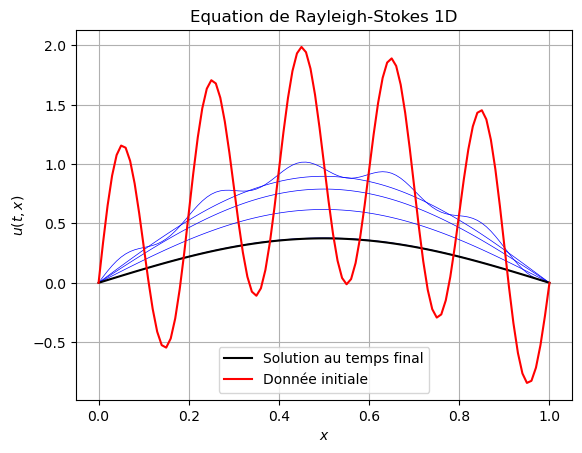
\includegraphics[width=\textwidth]{images/stabilite/alpha_dix_moins_5.png}
        \caption{$\alpha=10^{-5}$}
    \end{subfigure}
    \hfill
    \begin{subfigure}{0.32\textwidth}
        \centering
        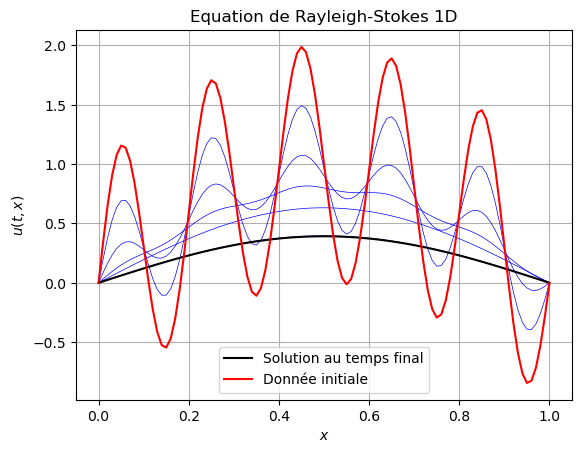
\includegraphics[width=\textwidth]{images/stabilite/alpha_dix_moins_2.png}
        \caption{$\alpha=5\times 10^{-3}$}
    \end{subfigure}
    \hfill
    \begin{subfigure}{0.32\textwidth}
        \centering
        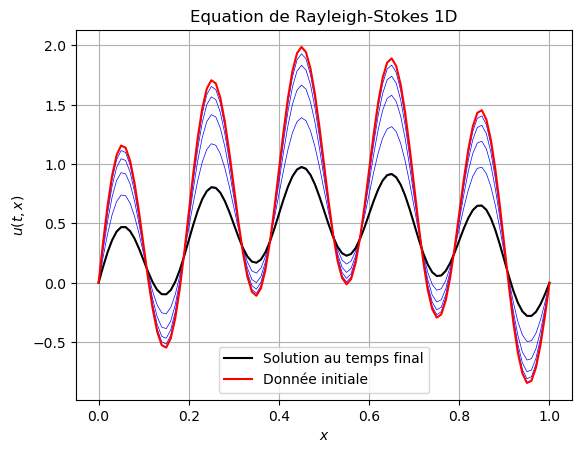
\includegraphics[width=\textwidth]{images/stabilite/alpha_dix_moins_1.png}
        \caption{$\alpha=10^{-1}$}
    \end{subfigure}
    \caption{Comportement des hautes fréquences en fonction de $\alpha$}
    \label{fig:stabilite_alpha}
\end{figure}
Sur la figure (a), on a $\alpha \ll \nu \Delta t$ et les hautes fréquences sont immédiatement amorties. Sur la figure (b), on a $\alpha \sim \nu \Delta t$, les hautes fréquences sont amorties mais cela prend plus de temps. Sur la figure (c), $\alpha \gg \nu \Delta t$, les hautes fréquences sont conservées. Cette exemple illustre parfaitement l'analyse précédente.

\subsubsection{Erreur globale et convergence}
Le schéma est consistant d'ordre un en temps et deux en espace, il est également stable en norme $L^2$, par conséquent la solution numérique converge vers la solution exacte. De plus, l'erreur globale est en $O(\Delta t +h^2)$.

\subsubsection{Conditionnement}
On va étudier le conditionnement de la matrice $A:=I-(\nu\Delta t+\alpha)\Delta_h$ pour mettre en évidence son impact dans la stabilisation du comportement numérique. La matrice est définie par
\begin{eqnarray*}
    I - (\nu\Delta t +\alpha)\Delta_h = \begin{pmatrix}
        1+2\frac{\nu \Delta t+\alpha}{h^2} & -\frac{\nu\Delta t + \alpha}{h^2} & 0  & \cdots & 0 \\
       -\frac{\nu\Delta t + \alpha}{h^2} & 1+2\frac{\nu \Delta t+\alpha}{h^2} & -\frac{\nu\Delta t + \alpha}{h^2}  & \ddots & \vdots \\
        0 & \ddots & \ddots & \ddots &  0 \\
        \vdots & \ddots & \ddots & \ddots &  -\frac{\nu\Delta t + \alpha}{h^2} \\
        0 & \cdots &  0 & -\frac{\nu\Delta t + \alpha}{h^2} & 1+2\frac{\nu \Delta t+\alpha}{h^2}
    \end{pmatrix}
\end{eqnarray*}
On va utiliser le théorème de Gerschgorin pour connaître le spectre de $A$. Les disques de Gerschgorin sont 
\begin{eqnarray*}
    D_1 = D_m &=& B\bigg(1+2\frac{\nu\Delta t+\alpha}{h^2}, \ \frac{\nu\Delta t+\alpha}{h^2}\bigg) \\
    \forall i \in \{2,\dots,m-1\}, \ D_i &=& B\bigg(1+2\frac{\nu\Delta t+\alpha}{h^2}, \ 2\frac{\nu\Delta t+\alpha}{h^2}\bigg)
\end{eqnarray*}
où $B(x, r)$ désigne la boule de centre $x$ et de rayon $r$ pour la norme euclidienne. Par le théorème de Gerschgorin, on a 
\begin{equation*}
    \mathrm{Sp}(A) \subset \bigcup_{i=1}^m D_i = B\bigg(1+2\frac{\nu\Delta t+\alpha}{h^2}, \ 2\frac{\nu\Delta t+\alpha}{h^2}\bigg)
\end{equation*}
or, $A$ est symétrique, donc diagonalisable à valeurs propres réelles. Ainsi, 
\begin{equation*}
    \mathrm{Sp}(A) \subset  \Big[1, \ 1+4\frac{\nu\Delta t+\alpha}{h^2}\Big]
\end{equation*}
De plus, $A$ est irréductible car son graphe est connexe donc si $\lambda$ est une valeur propre de $A$, on a 
\begin{eqnarray*}
    \lambda \in \bigcup_{i=1}^m \partial D_i &\Longrightarrow& \lambda \in 
    \bigcap_{i=1}^m \partial D_i = \emptyset
\end{eqnarray*}
On peut donc affiner notre localisation du spectre de $A$
\begin{equation*}
    \mathrm{Sp}(A) \subset \  \Big]1, \ 1+4\frac{\nu\Delta t+\alpha}{h^2}\Big[ \ \setminus \Big\{1+\frac{\nu\Delta t+\alpha}{h^2}, 1+3\frac{\nu\Delta t+\alpha}{h^2} \Big\}
\end{equation*}
On en déduit 
\begin{eqnarray*}
    \lambda_1 := \min_{\lambda \in \mathrm{Sp}(A)} \lambda > 1 \ \ \ &\text{ et }& \ \ \ \lambda_m :=\max_{\lambda \in \mathrm{Sp}(A)} \lambda < 1+4\frac{\nu\Delta t+\alpha}{h^2}
\end{eqnarray*}
Finalement,
\begin{equation*}
    \mathrm{cond}(A) = \frac{\lambda_m}{\lambda_1} < 1+4\frac{\nu \Delta t +\alpha}{h^2}
\end{equation*}
Donc, si on choisit $\alpha$ et $\Delta t$ tels que $\nu \Delta t \ll \alpha$ alors 
\begin{equation*}
    \mathrm{cond}(A) \leq 1 + \frac{\alpha}{h^2}
\end{equation*}
Le conditionnement de $A$ devient indépendant de $\Delta t$ ce qui permet de faire varier librement le pas de temps sans influer sur la stabilité numérique du schéma.
\begin{remark}
     Si on veut que le conditionnement de la matrice $A$ soit indépendant du choix de $\Delta t$ on doit choisir $\nu \Delta t \ll \alpha$, or on a vu lors de l'étude de la stabilité du schéma que pour avoir un effet de filtre passe-bas on devait choisir $\nu \Delta t \gg \alpha$. En pratique, on privilégiera la propriété de filtre passe-bas tout en faisant attention à ce que cela ne limite pas notre façon de résoudre le système linéaire $AX=Y$.
\end{remark}

\subsection{Comparaison avec l'équation de la chaleur}
Dans cette section, on veut comparer le schéma d'Euler implicite entre l'équation de Rayleigh-Stokes et l'équation de la chaleur. On considère les problèmes aux limites suivants
\begin{itemize}
    \item Problème aux limites pour l'équation de Rayleigh-Stokes
    \begin{equation*}
        \begin{cases}
            \partial_tu(t,x) - \nu\partial_{xx} u(t,x) - \alpha\partial_{xx} \big(\partial_t u(t,x)\big) = 0 & \forall (t,x) \in \ ]0, 1[ \ \times \ ]0,1[  \\
            u(0,x) = u_0(x) = \sin{(\pi x)} & \forall x \in \ ]0,1[ \\
            u(t, 0) = u(t,1) = 0 & \forall t \in \ ]0,1[
        \end{cases}
    \end{equation*}
    La solution de ce problème est donnée par 
    \begin{equation}\label{compRSchaleur_solRS}
        u_{\text{RS}}(t,x) = \sin{(\pi x)}\exp{\Big( -\frac{\nu \pi^2}{1+\alpha \pi^2}t\Big)}
    \end{equation}
    \item Problème aux limites pour l'équation de la chaleur
    \begin{equation*}
        \begin{cases}
            \partial_tu(t,x) - \nu\partial_{xx} u(t,x) = 0 & \forall (t,x) \in \ ]0,1[ \ \times \ ]0,1[  \\
            u(0,x) = u_0(x)=\sin{(\pi x)} & \forall x \in \ ]0,1[ \\
            u(t, 0) = u(t,1) = 0 & \forall t \in \ ]0,1[
        \end{cases}
    \end{equation*}
    La solution de ce problème est donnée par 
    \begin{equation}\label{compRSchaleur_solchaleur}
        u_{\text{chal}}(t,x) = \sin{(\pi x)}\exp{(-\nu \pi^2t)}
    \end{equation}
\end{itemize}
L'objectif ici est d'observer l'influence du paramètre $\alpha$ sur la dissipation de l'énergie cinétique et de comparer ce phénomène avec l'équation de la chaleur (cas $\alpha=0$). Pour nos simulations, on choisit $\nu = 0.1$, et $h=\Delta t = \dfrac{1}{100}$. La simulation pour l'équation de la chaleur donne le résultat suivant
\begin{figure}[!ht]
    \centering
    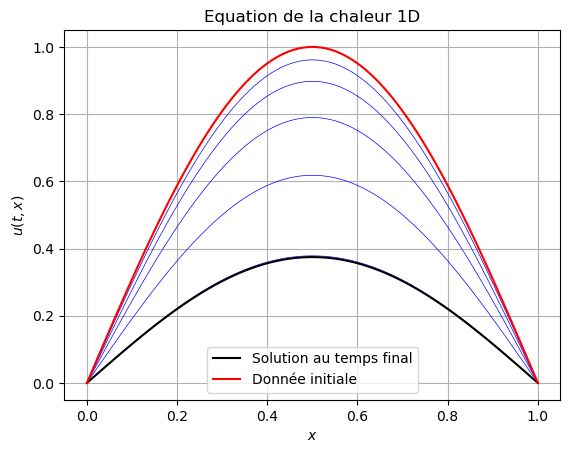
\includegraphics[width=0.5\linewidth]{images/comparaison_chaleur/eq_chaleur.png}
    \caption{\'Equation de la chaleur $1$D pour l'évolution temporelle du profil de vitesse $u(t,x)$ pour un mode sinusoïdal}
    \label{fig:eqchaleur}
\end{figure}
\\
Pour comparer à l'équation de Rayleigh-Stokes, on choisit $\alpha \in \{5\times 10^{-1}, 5 \times 10^{-2}, 5 \times 10^{-4}\}$, voici les résultats des simulations
\begin{figure}[!ht]
    \centering
    \begin{subfigure}{0.32\textwidth}
        \centering
        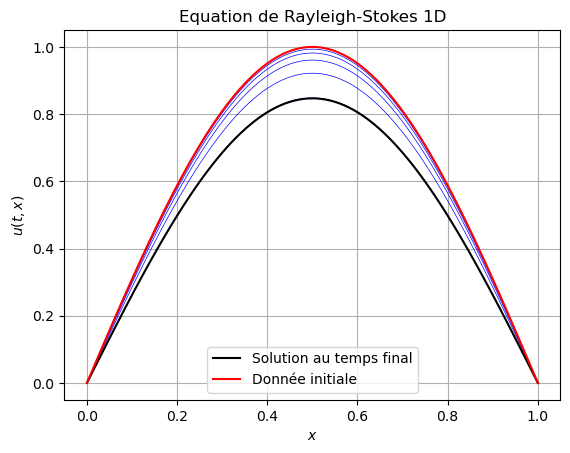
\includegraphics[width=\textwidth]{images/comparaison_chaleur/eq_RS_alpha1.png}
        \caption{$\alpha=5\times 10^{-1}$}
    \end{subfigure}
    \hfill
    \begin{subfigure}{0.32\textwidth}
        \centering
        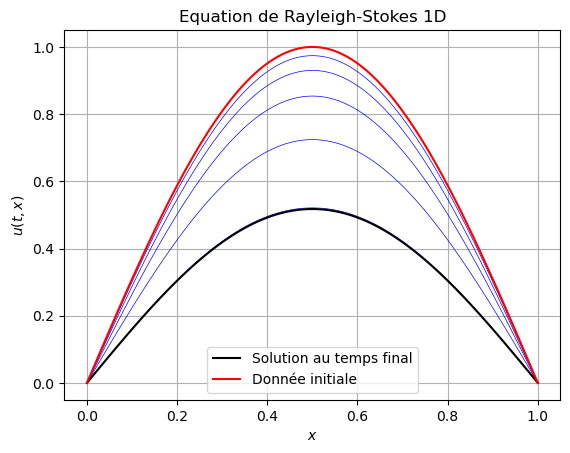
\includegraphics[width=\textwidth]{images/comparaison_chaleur/eq_RS_alpha2.png}
        \caption{$\alpha=5\times 10^{-2}$}
    \end{subfigure}
    \hfill
    \begin{subfigure}{0.32\textwidth}
        \centering
        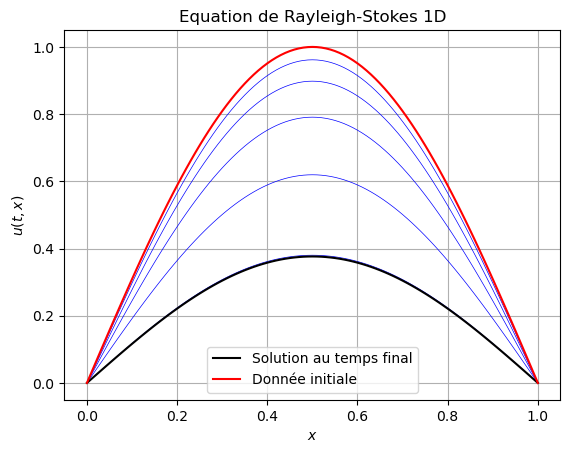
\includegraphics[width=\textwidth]{images/comparaison_chaleur/eq_RS_alpha3.png}
        \caption{$\alpha=5 \times 10^{-4}$}
    \end{subfigure}
    \caption{Influence du paramètre $\alpha$ sur la dissipation de l'énergie pour l'équation de Rayleigh-Stokes $1$D}
    \label{fig:comparaisonchaleurRS}
\end{figure}
\\
On remarque que sur la figure \ref{fig:eqchaleur}, le profil sinusoïdal est très rapidement amorti. Physiquement, c'est une diffusion classique du fluide, le mouvement du fluide va s'arrêter rapidement. Analytiquement, la solution est donnée par \eqref{compRSchaleur_solchaleur} avec 
\begin{equation*}
    \nu \pi^2 \approx 0.99
\end{equation*}
on a une décroissance exponentielle ce qui explique l'amortissement rapide du profil sinusoïdal.
Sur les figures \ref{fig:comparaisonchaleurRS}, on observe plusieurs cas en fonction de la valeur du paramètre $\alpha$. Le paramètre $\alpha$ est un paramètre de viscoélasticité du fluide, il va donc agir comme une contrainte supplémentaire sur le fluide et ralentir plus ou moins la diffusion. 
Sur la figure (a) de \ref{fig:comparaisonchaleurRS}, $\alpha$ est grand (dans le sens de l'ordre de $\nu$) et on observe que le profil sinusoïdal n'est presque pas amorti. La diffusion est donc ralentie par le paramètre $\alpha$. Si on regarde la solution \eqref{compRSchaleur_solRS} dans cette configuration, on a 
\begin{equation*}
    \frac{\nu \pi^2}{1+\alpha \pi^2} \approx 0.17
\end{equation*}
La décroissance exponentielle est fortement ralentie par la présence du terme $\alpha$ grand.
Sur la figure (b) de \ref{fig:comparaisonchaleurRS}, $\alpha$ est plus petit, le profil sinusoïdal est amorti mais toujours plus lentement que pour l'équation de la chaleur. Ici, on a 
\begin{equation*}
    \frac{\nu \pi^2}{1+\alpha \pi^2} \approx 0.66
\end{equation*}
On retrouve à nouveau l'influence du paramètre $\alpha$ sur la décroissance exponentielle du profil.
Enfin sur la figure (c) de \ref{fig:comparaisonchaleurRS}, $\alpha$ est négligeable devant $\nu$ et on retrouve un amortissement du profil comme pour l'équation de la chaleur \ref{fig:eqchaleur}. Ici, on a
\begin{equation*}
    \frac{\nu \pi^2}{1+\alpha \pi^2} \approx 0.98
\end{equation*}
La contrainte physique liée au paramètre $\alpha$ est très faible, c'est donc le caractère diffusif qui va prendre le dessus.
    
\subsection{Quelques exemples}
\subsubsection{La fonction indicatrice}
Pour ce premier cas on s’intéresse au problème suivant:
   \begin{equation*}
        \begin{cases}
            \partial_tu(t,x) - \nu\partial_{xx} u(t,x) - \alpha\partial_{xx} \big(\partial_t u(t,x)\big) = 0 & \forall (t,x) \in \ ]0, T[ \ \times \ ]0,L[  \\
            u(0,x) = u_0(x) = \mathds{1}_{\left[\tfrac{L}{4},\tfrac{3L}{4}\right]}(x) & \forall x \in \ ]0,L[ \\
            u(t, 0) = u(t,L) = 0 & \forall t \in \ ]0,T[
        \end{cases}
    \end{equation*}
Après une décomposition en série de Fourier la solution est donnée par
\begin{eqnarray*}
    u(t,x) = \sum_{k=1}^{N} c_k \exp\left(-\frac{\nu\lambda_k}{1+\alpha\lambda_k}\,t\right)\sin\left(\frac{k\pi x}{L}\right)
\end{eqnarray*}
avec 
\begin{equation*}
    c_k = \frac{2}{k\pi}\left(\cos(\frac{k\pi}{4}) -\cos(\frac{3k\pi}{4})\right)
\end{equation*}
Cette décomposition repose sur le fait que notre fonction initial peut s'écrire comme une série composé de sinus sur $[0,L]$
\begin{eqnarray*}
    u_0(x) = \sum_{k=1}^{\infty} c_k \sin\left(\frac{k\pi x}{L}\right)
\end{eqnarray*}
En multipliant par $\sin\Big(\dfrac{j\pi x}{L}\Big)$ de chaque côté et intégrant sur $[0,L]$ cela nous permet d'identifier $c_k$. \\
On résout numériquement le problème en posant $N = 200$, $L=10$ et $T=20$. Pour les paramètre de l'équation de Rayleigh-Stokes on choisi $\nu = 0.4$ et $\alpha=0.5$ Cela va nous permettre d'étudier comment varie notre solution initial et quels sont les effets du paramètre $\alpha$.  
\begin{figure}[!ht]
    \centering
    \begin{subfigure}{0.48\textwidth}
        \centering
        \includegraphics[width=\textwidth]{images/Exemples/Indicatrice/resolution_indicatrice.png}
        \caption{Évolution de la solution}
    \end{subfigure}
    \hfill
    \begin{subfigure}{0.48\textwidth}
        \centering
        \includegraphics[width=\textwidth]{images/Exemples/Indicatrice/comparaison_final_theorique_indicatrice.png}
        \caption{Comparaison solution finale/théorique}
    \end{subfigure}
    \caption{ Résolution de l'équation de Rayleigh-Stokes $1$D}
    \label{fig:Exemples_RS_Stokes_indicatrice}
\end{figure}
\begin{figure}[H]
    \centering
    \includegraphics[width=\linewidth]{images/Exemples/Indicatrice/comparaison alpha indicatrice.png}
    \caption{Comparaison en fonction de alpha}
    \label{Indicatrice_comparaisons des alpha}
\end{figure}
On observe sur la figure \eqref{fig:Exemples_RS_Stokes_indicatrice} que la solution initial discontinue est rapidement lissé et amorti cela correspond bien aux résultats observés précédemment.

La figure \eqref{Indicatrice_comparaisons des alpha} illustre l'influence du paramètre
$\alpha$ : pour $\alpha$ grand, le fluide résiste davantage au changement
et conserve plus longtemps la mémoire de son état initial.

\subsubsection{Problème de Stokes impulsif, démarrage brusque d’une paroi}
On va maintenant simuler la réponse d'un fluide à l'accélération d'une paroi. On se place dans un canal de largeur $L=1$ au temps initial $t=0$. On suppose qu'au temps initial le fluide est au repos. On impose ensuite une vitesse constante $U_0$ sur le bord $x=0$, ici on prendra $U_0=10$. Le problème s'écrit alors:
\begin{equation*}
    \begin{cases}
        \partial_tu(t,x) - \nu\partial_{xx} u(t,x) - \alpha\partial_{xx} \big(\partial_t u(t,x)\big) = 0 & \forall (t,x) \in \ ]0, 5[ \ \times \ ]0,1[  \\
        u(0,x) = u_0(x) = 0 & \forall x \in \ ]0,1[ \\
        u(t,1) = 0 & \forall t \in \ ]0,5[ \\
        u(t,0) = U_0 & \forall t \in \ ]0,5[
    \end{cases}
\end{equation*}
Le problème n'ayant plus des conditions de Dirichlet homogène il faut faire un relèvement. On pose $u = \Tilde{u} + g$ avec $\Tilde{u} \in H^1_0([0,1])$  et $g(x) = U_0 \Big(1 - \dfrac{x}{L}\Big)$ de sorte que $g(1)=0$ et $g(0) = U_0$.
La formulation variationnelle reste la même que dans le cas homogène, il faut juste prendre en compte la fonction $g$ dans les conditions initiales et dans la solution du problème. On obtient le résultat suivant
\begin{figure}[!ht]
    \centering
    \begin{subfigure}{0.32\textwidth}
        \centering
        \includegraphics[width=\textwidth]{images/Exemples/Plaque en mouvement/RS_EI_plaque_1.png}
        \caption{$\alpha=0.1$}
    \end{subfigure}
    \hfill
    \begin{subfigure}{0.32\textwidth}
        \centering
        \includegraphics[width=\textwidth]{images/Exemples/Plaque en mouvement/RS_EI_plaque_2.png}
        \caption{$\alpha=0.5$}
    \end{subfigure}
    \hfill
    \begin{subfigure}{0.32\textwidth}
        \centering
        \includegraphics[width=\textwidth]{images/Exemples/Plaque en mouvement/RS_EI_plaque_3.png}
        \caption{$\alpha=0.9$}
    \end{subfigure}
    \caption{Influence du paramètre $\alpha$ sur la résistance du fluide face à la condition initiale pour l'équation de Rayleigh-Stokes $1$D}
    \label{fig:Exemples_RS_Stokes_impulsif}
\end{figure} \\
On peut remarquer que sur les 3 cas précédents le terme en $\alpha$ joue un rôle sur l'accélération de la vitesse. Si $\alpha$ est petit alors le profil du fluide rejoint rapidement le profil de Couette alors que pour une grande valeur on va avoir besoin de beaucoup plus de temps pour rejoindre le profil final. Le terme $\alpha$ joue un rôle de \og mémoire \fg{}, le fluide résiste au changement pour garder son état initial. \\
Ce genre de propriétés s'avèrent importantes dans le monde industriel où ce genre de mouvement peu avoir lieu lors du démarrage de système de pompage d'un fluide complexe. Si le fluide subit une accélération rapide il faut être capable de savoir à quel point il résistera car s'il est très visqueux cela entraînera des contraintes de cisaillement élevés qui pourraient abîmer les parois de la machine.

\subsubsection{Régime forcé et analyse du déphasage viscoélastique}
%T = 4 
%v = 0.4
%alpha = 0.6
%L = 10
%Nx = 500
%omega = 0.5 
%A = 2 
%alpha1 = (np.pi / L)**2
%phi = np.arctan2(gamma * (1 + alpha * alpha1), v * alpha1)
Ce cas test étudie la réponse du fluide à une sollicitation externe périodique. Contrairement aux tests précédents, ici il y a un terme source et nous regardons l’établissement d’un cycle limite stationnaire, mais pas immobile. L'équation de Rayleigh-Stokes s'écrit. 
\begin{eqnarray}\label{RS_exemple_dephasage}
    \partial_tu(t,x) - \nu \partial_{xx}u(t,x) - \alpha \partial_{txx}u(t,x) = A \sin(\omega t)\sin\Big(\frac{\pi x}{L}\Big)
\end{eqnarray}
Le paramètre $A$ correspond à l'amplitude et $\omega$ à la pulsation. On pose d'abord $L= 10, \ A=5 \text{ et } \omega = 0.7$. On cherche à résoudre le problème jusqu'au temps $T=4$ pour $\nu = 0.4 \text{ et } \alpha=0.5$.
Calculons la solution exacte pour comparer avec notre schéma. On procède par séparation de variable et on cherche une solution de la même forme
\begin{eqnarray*}
    u(t,x) = v(t) \sin\Big(\frac{\pi x}{L}\Big)
\end{eqnarray*}
En calculant les dérivées partielles et en notant $\lambda_1 := \Big(\dfrac{\pi}{L} \Big)^2$ on peut réécrire \eqref{RS_exemple_dephasage}
\begin{equation*}
    v'(t) \sin\Big(\frac{\pi x}{L}\Big) + \nu \lambda_1 v(t)\sin\Big(\frac{\pi x}{L}\Big) + \alpha \lambda_1 v'(t)\sin\Big(\frac{\pi x}{L}\Big) = A\sin(\omega t)\sin\Big(\frac{\pi x}{L}\Big)
\end{equation*}
Comme pour tout $x \in \ ]0,L[$, $\sin\Big(\dfrac{\pi x}{L}\Big) \neq 0$, on peut simplifier et ainsi obtenir
\begin{equation*}
    (1 + \alpha \lambda_1)v'(t) + \nu \lambda_1v(t) = A \sin(\omega t)
\end{equation*}
On cherche une solution particulière de cette EDO sous la même forme que le second membre
\begin{equation*}
    v(t) = P \sin(\omega t) + Q\cos(\omega t) \ \ \ \ \ \text{ où } P, Q \in \bbR
\end{equation*}
Alors 
\begin{equation*}
    v'(t) = \omega P \cos(\omega t) - \omega Q\sin(\omega t)
\end{equation*}
On trouve alors $P = \dfrac{\nu \lambda_1 A}{D}$ et $Q= - \dfrac{(1 + \alpha \lambda_1)\omega A}{D}$ où $D := (1+\alpha \lambda_1) + (\nu \lambda_1)^2$.
Puis, en utilisant la propriété trigonométrique
\begin{eqnarray} \label{trigo_equation_exemple}
    \sin(\omega t - \varphi) = \cos(\varphi)\sin(\omega t) - \sin(\varphi)\cos(\omega t)
\end{eqnarray}
on identifie 
\begin{eqnarray*}
    \frac{\nu \lambda_1 A}{D} = \cos(\varphi) \ \ \  &\text{ et }& \ \ \ \frac{(1 + \alpha \lambda_1)\omega A}{D}= \sin(\varphi)
\end{eqnarray*}
d'où 
\begin{equation*}
    \varphi= \arctan \bigg(\frac{(1+\alpha \lambda_1) \omega}{\nu \lambda_1}\bigg)
\end{equation*}
De plus en multipliant \eqref{trigo_equation_exemple} par $U(\omega)$ on trouve que $U$ doit vérifier $U(\omega) = \sqrt{P^2 + Q^2}$. Finalement on obtient une solution 
\begin{equation*}
    v(t) = C \exp{\Big(-\frac{\nu \lambda_1}{1+ \alpha \lambda_1}t\Big)} + U(\omega)\sin(\omega t-\varphi) \ \ \ \ \ \text{ où } C \in \bbR
\end{equation*}
En supposant que le fluide est au repos à l'état initial, c'est-à-dire $u_0 = 0$ on trouve 
\begin{equation*}
    C = -U(\omega) \sin(-\varphi) = U(\omega) \sin(\varphi)
\end{equation*}
Donc $v(t)$ s'écrit
\begin{equation*}
    v(t) = U(\omega) \sin(\varphi) \exp{\Big(-\frac{\nu \lambda_1}{1+ \alpha \lambda_1}t\Big)} + U(\omega)\sin(\omega t-\varphi)
\end{equation*}
Ce qui nous permet d'écrire la solution
\begin{equation*}
    u(t,x) = \bigg(U(\omega) \sin(\varphi) \exp{\Big(-\frac{\nu \lambda_1}{1+ \alpha \lambda_1}t\Big)} + U(\omega)\sin(\omega t-\varphi) \bigg) \sin\Big(\frac{\pi x}{L}\Big)
\end{equation*}
En temps long on remarque que l'exponentielle tend vers $0$. On simplifiera alors la solution en 
\begin{equation*}
    u(t,x) = U(\omega)\sin(\omega t-\varphi)  \sin\Big(\frac{\pi x}{L}\Big)
\end{equation*}
On peut alors étudier cette équation en fonction des paramètres $\alpha$ et $\omega$. La résolution numérique donne les résultats suivant:
\begin{figure}[H]
    \centering
    \begin{subfigure}{0.47\textwidth}
        \centering
        \includegraphics[width=\textwidth]{images/Exemples/Dephasage viscoelastique/RS_dephasage.png}
        \caption{$\alpha=0.5$}
    \end{subfigure}
    \hfill
    \begin{subfigure}{0.47\textwidth}
        \centering
        \includegraphics[width=\textwidth]{images/Exemples/Dephasage viscoelastique/RS_dephasage final.png}
        \caption{$\alpha=0.5$}
    \end{subfigure}
    \hfill
    \caption{Analyse d'un régime forcé pour l'équation de Rayleigh-Stokes $1$D}
    \label{fig:Exemples_RS_Stokes_régime_forcé}
\end{figure} 
\begin{figure}[H]
    \centering
    \begin{subfigure}{0.47\textwidth}
        \centering
        \includegraphics[width=\textwidth]{images/Exemples/Dephasage viscoelastique/RS_convergence_temps_dephasage.png}
        \caption{Ordre de convergence}
    \end{subfigure}
    \hfill
    \begin{subfigure}{0.47\textwidth}
        \centering
        \includegraphics[width=\textwidth]{images/Exemples/Dephasage viscoelastique/Amplitude de la reponse.png}
        \caption{Variation théorique}
    \end{subfigure}
    \hfill
    \caption{Étude de la convergence en temps et de l'évolution de l’amplitude pour l'équation de Rayleigh-Stokes $1$D} \label{fig:Exemples_RS_Stokes_régime_forcé_comparaison_final}
\end{figure} 
\begin{figure}[H]
    \centering
    \begin{subfigure}{0.47\textwidth}
        \centering
        \includegraphics[width=\textwidth]{images/Exemples/Dephasage viscoelastique/Amplitude alpha.png}
        \caption{Évolution de l'amplitude en fonction de $\alpha$ }
    \end{subfigure}
    \hfill
    \begin{subfigure}{0.47\textwidth}
        \centering
        \includegraphics[width=\textwidth]{images/Exemples/Dephasage viscoelastique/Amplitude_omega.png}
        \caption{Amplitude numérique en fonction de $\omega$}
    \end{subfigure}
    \hfill
    \caption{Étude de l’amplitude pour l'équation de Rayleigh-Stokes $1$D}
    \label{fig:Exemples_RS_Stokes_régime_forcé_amplitude}
\end{figure} 

Sur les dernières images on a mis en évidence que le paramètre $\omega$ influe fortement sur l'évolution de l'amplitude de la vitesse du fluide, contrairement au paramètre $\alpha$ qui lui à un effet plus modéré. Ce sont des propriétés similaires de filtres passe bas que nous avions trouvé précédemment. Plus $\omega$ est grand plus la pulsation est importante et donc la fréquence est élevée. Or l'amplitude est plus atténuée, les hautes fréquences sont filtrées.
\newpage
\subsection{Un autre schéma}
Dans cette section, on va chercher à augmenter la précision en temps de notre schéma, pour ça on s'intéresse au schéma de Crank-Nicolson. Pour ça, on repart de l'équation \eqref{schema_semi_discret}, on intègre entre deux instants $t_n$, $t_{n+1}$ et on utilise cette fois la méthode des trapèzes pour approximer les intégrales. Ce qui nous donne après avoir divisé par $\Delta t$
\begin{eqnarray}\label{schemaCN1}
    \frac{u_i^{n+1}-u_i^n}{\Delta t} &-& \frac{\nu}{2} \bigg( \frac{u_{i-1}^{n+1}-2u_i^{n+1}+ u_{i+1}^{n+1}}{h^2} + \frac{u_{i-1}^{n}-2u_i^{n}+u_{i+1}^{n}}{h^2} \bigg) \\
    &-& \frac{\alpha}{\Delta t}\bigg( \frac{u_{i-1}^{n+1}-2u_i^{n+1}+u_{i+1}^{n+1}}{h^2} 
    -\frac{u_{i-1}^{n}-2u_i^{n}+u_{i+1}^{n}}{h^2}\bigg) = f_i \nonumber
\end{eqnarray}
%Puisque nous avons réalisé notre étude à partir du schéma d'Euler implicite, il est facile de retrouver plusieurs propriétés importantes du schéma de Crank-Nicolson qui est construit en faisant un moyenne du schéma d'Euler implicite et explicite. \\
%Le schéma d'Euler implicite donnait :
%\begin{eqnarray*}
%    \frac{U^{n+1} - U^n}{\Delta t} - \nu \Delta _h U^{n+1} - \alpha\bigg(\frac{\Delta_h U^{n+1} - \Delta_h U^n}{\Delta t} \bigg) = F
%\end{eqnarray*}
%Le schéma d'Euler explicite s'écrit alors simplement :
%\begin{eqnarray*}
%    \frac{U^{n+1} - U^n}{\Delta t} - \nu \Delta _h U^{n} - \alpha\bigg(\frac{\Delta_h U^{n+1} - \Delta_h U^n}{\Delta t} \bigg) = F
%\end{eqnarray*}
Avec les notations introduites dans la section sur le schéma d'Euler implicite, on peut réécrire l'équation précédente de la façon suivant
\begin{equation*}
    \frac{U^{n+1} - U^n}{\Delta t} - \frac{\nu}{2} \big(\Delta _h U^{n+1}-\Delta_hU^n\big) - \alpha\bigg(\frac{\Delta_h U^{n+1} - \Delta_h U^n}{\Delta t} \bigg) = F
\end{equation*}
Finalement, en isolant l'inconnue au temps $n+1$ et au temps $n$ on peut écrire le système final
\begin{eqnarray*}
    \Big(I - \Big( \frac{\nu \Delta t}{2} + \alpha \Big)\Delta_h\Big)  U^{n+1} = \Big(I + \Big(\frac{\nu \Delta t}{2} - \alpha\Big) \Delta_h\Big) U^n + \Delta t F
\end{eqnarray*}

\subsubsection{Consistance}
Le schéma de Crank-Nicolson est consistant d'ordre deux en temps et en espace. Comme dans la section sur le schéma d'Euler implicite on montre cela par un calcul avec des développements limités. On pose
\begin{eqnarray*}
    A &:=& \frac{u(t+\Delta t,x)-u(t,x)}{\Delta t} \\
    B &:=& \frac{\nu}{2}\bigg(\frac{u(t+\Delta t,x-h)-2u(t+\Delta t, x)+ u(t+\Delta t, x+h)}{h^2} \\
    &+& \frac{u(t,x-h)-2u(t, x) + u(t, x+h)}{h^2}\bigg) \\
    C &:=&\frac{\alpha}{\Delta t}\bigg(\frac{u(t+\Delta t,x-h)-2u(t+\Delta t, x) + u(t+\Delta t, x+h)}{h^2} \\
    &-&\frac{u(t,x-h)-2u(t, x)+u(t, x+h)}{h^2}\bigg) \\
    \calL_hu(t,x) &=& A - B - C 
\end{eqnarray*}
Comparé au schéma d'Euler implicite, seul le terme $B$ est modifié, on utilise donc nos calculs précédents et on effectue le développement limité du terme supplémentaire dans l'expression de $B$. Ce qui donne
\begin{eqnarray*}
    A &=& \partial_{t}u(t,x) - \frac{\Delta t}{2} \partial_{tt}u(t,x) + O(\Delta t^2) \\
    B &=&  \frac{\nu}{2} \Big(\partial_{xx}u(t,x) + \Delta t \partial_{xxt}u(t,x) + \frac{h^2}{12} \partial_{xxxx}u(t,x) + O(\Delta t^2+h^3)\Big) \\
    &+& \frac{\nu}{2} \Big(\partial_{xx}u(t,x) + \frac{h^2}{12} \partial_{xxxx}u(t,x) + O(h^3)\Big) \\
    C &=& \alpha\Big(\partial_{xxt}u(t,x) + \frac{h^2}{12}\partial_{xxxxt}u(t,x) - \frac{\Delta t}{2}\partial_{xxtt}u(t,x) - \frac{h^2\Delta t}{24}\partial_{xxxxtt}u(t,x) \\
    &+& O(\Delta t^2 + h^3)\Big)   
\end{eqnarray*}
D'où 
\begin{eqnarray*}
    \calL_hu -\calL u &=& -\frac{\Delta t}{2}\partial_{tt}u + \nu\frac{\Delta t }{2} \partial_{xxt}u+ \alpha\frac{\Delta t }{2} \partial_{xxtt}u  + O(\Delta t^2 + h^2)
\end{eqnarray*}
On utilise notre EDP
\begin{eqnarray*}
    \partial_tu = \nu \partial_{xx}u + \alpha \partial_{xxt}u 
    & \Longrightarrow& 
    \partial_{tt}u = \nu \partial_{xxt}u + \alpha \partial_{xxtt}u
\end{eqnarray*}
L'erreur de troncature se simplifie alors en
\begin{eqnarray*}
    \calL_hu -\calL u &=& -\frac{\Delta t}{2}(\nu \partial_{xxt}u + \alpha \partial_{xxtt}u) + \nu\frac{\Delta t }{2} \partial_{xxt}u+ \alpha\frac{\Delta t }{2} \partial_{xxtt}u  + O(\Delta t^2 + h^2) \\
    &=& O(\Delta t^2 + h^2)
\end{eqnarray*}
Le schéma est bien d'ordre deux en temps et en espace.

\subsubsection{Stabilité}
On utilise les notations introduites à la section \ref{Stabilité_EI}. Tout comme le schéma d'Euler implicite ce schéma vérifie les conditions de stabilité de Von Neumann. En effet, on part de \eqref{schemaCN1} et en réalisant exactement les mêmes calculs qu'à la section \eqref{Stabilité_EI}, on obtient
\begin{eqnarray*}
    \Big(1+\Big(\alpha +\frac{\nu \Delta t}{2}\Big) \frac{4}{h^2}\sin^2(\pi k h)\Big)\hat{u}^{n+1}(k) &=& \Big(1+\Big(\alpha - \frac{\nu \Delta t}{2}\Big) \frac{4}{h^2}\sin^2(\pi kh)\Big)\hat{u}^{n}(k)
\end{eqnarray*}
Le facteur d'amplification de ce schéma s'écrit alors
\begin{eqnarray*}
    \mathscr{A}(k \ ; \Delta t ,h) &=& \frac{1+\Big(\alpha - \dfrac{\nu \Delta t}{2}\Big) \dfrac{4}{h^2}\sin^2(\pi kh)}{1+\Big(\alpha +\dfrac{\nu \Delta t}{2}\Big) \dfrac{4}{h^2}\sin^2(\pi kh) }
\end{eqnarray*}
On pose $a=\alpha \dfrac{4}{h^2}\sin^2(\pi kh)$ et $b=\dfrac{\nu \Delta t}{2}\dfrac{4}{h^2}\sin^2(\pi kh)$, comme $\alpha, \ \nu, \ h, \ \Delta t >0$ on a $a, \ b >0$. Le facteur d'amplification s'écrit alors
\begin{eqnarray*}
    \scrA(k \ ; \Delta t ,h) &=& \frac{1+a-b}{1+a+b}
\end{eqnarray*}
on cherche à savoir si $|\scrA(k \ ; \Delta t ,h)| \leq 1$, donc si 
\begin{eqnarray*}
    \bigg|\frac{1+a-b}{1+a+b}\bigg| \leq 1 &\Longrightarrow& |1+a-b| \leq 1+a+b
\end{eqnarray*}
ce qui nous donne deux conditions
\begin{eqnarray*}
    1+a-b < 1+a+b \ \ \ &\text{ ou }& \ \ \ -1-a-b < 1+a-b \\
    0 < 2b \ \ \ &\text{ ou }& \ \ \ 0 < 2(1+a)
\end{eqnarray*}
ces deux conditions sont toujours vérifiées donc,
\begin{eqnarray*}
    \sup_{k \in \mathbb{Z}} \ |\mathscr{A}(k \ ; \Delta t ,h)| &\leq& 1
\end{eqnarray*}
Le schéma est donc stable en temps long et inconditionnellement stable en norme $L^2$.
On remarquera que contrairement aux schéma d'Euler implicite il est possible d'obtenir un facteur d'amplification négatif avec $\alpha < \dfrac{\nu \Delta t}{2}$.
% A voir ce que ça veut dire j'ai pas creusé plus. On devrait demander à Marche.

\subsubsection{Erreur globale et convergence}
Le schéma est consistant d'ordre deux en temps et en espace, il est également stable en norme $L^2$, par conséquent la solution numérique converge vers la solution exacte. De plus, l'erreur globale est en $O(\Delta t^2 +h^2)$.

\subsubsection{Comparaison avec le schéma d'Euler implicite}
On va implémenter un cas simple afin de mettre en évidence la différence de précision en temps du schéma d'Euler implicite et de celui de Crank-Nicolson. Pour ça, on choisit $L=\nu = T = 1$, $\alpha = 0.1$, $h=\dfrac{1}{500}$. On prend 
\begin{equation*}
    \Delta t \in \Big\{\frac{1}{10}, \frac{1}{20}, \frac{1}{40}, \frac{1}{80}, \frac{1}{160}\Big\}
\end{equation*}
Enfin, on choisit $u_0(x) = \sin(\pi x)$ comme donnée initiale. Dans ces conditions, notre solution exacte est définie par
\begin{equation*}
    u(t,x) = \exp\Big(\frac{-\pi^2t}{1+\alpha \pi^2}\Big)\sin(\pi x)
\end{equation*}
On obtient le graphique suivant
\begin{figure}[!ht]
    \centering
    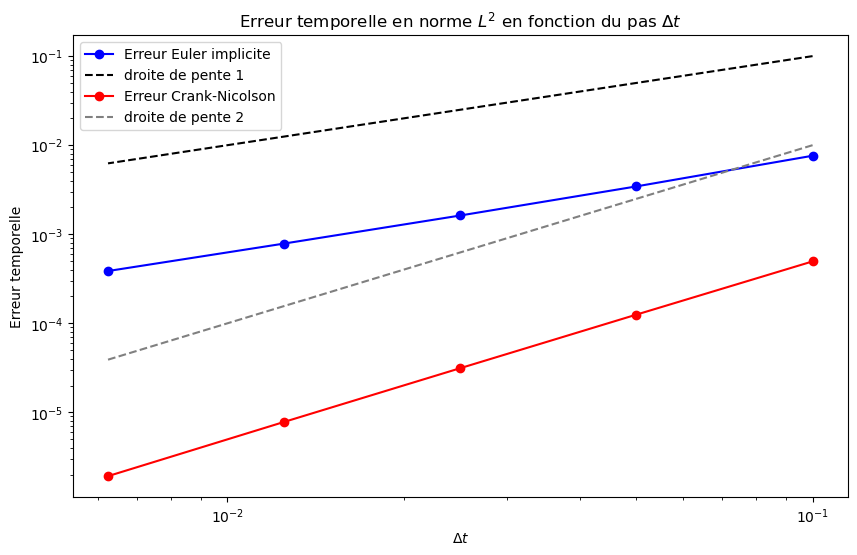
\includegraphics[width=\linewidth]{images/Crank-Nicolson/erreur_EI_CN.png}
    \caption{Comparaison Euler implicite et Crank-Nicolson}
    \label{fig:comparaison}
\end{figure}
\\\\
Ce graphique confirme nos résultats théoriques, le schéma d'Euler implicite est bien d'ordre $1$ en temps, celui de Crank-Nicolson est d'ordre $2$ en temps, il est donc plus précis que le schéma d'Euler implicite.

\newpage